\subsubsection{Sprint goal}

\subsubsection{Backlog}
\userstory%
{Come spettatore de \#leredita\\voglio raccogliere i tweet di chi prova a indovinare la ghigliottina,\\per visualizzare, in ordine temporale, tutti coloro che provano ad indovinare.}%
{5\\(2 frontend + 3 backend)}%
{Possibilità di visualizzare una pagina con tutti i tweet di tutte le persone che usano l'\#leredita e provano ad indovinare la ghigliottina.}%
{Cercando per data, verificare che vengano visualizzati i tentativi del giorno}

\userstory%
{Come spettatore de \#leredita\\voglio visualizzare, su una mappa, la posizione di tutti coloro che provano ad indovinare\\per conoscere la posizione di giocatori.}%
{4\\(4 frontend)}%
{Possibilità di visualizzare una pagina con tutte le posizioni su una mappa di tweet di tutte le persone che usano l'\#leredita e provano ad indovinare la ghigliottina.}%
{Manualmente verificare che nella mappa siano presenti i marker dei tweet con la geolocalizzazione}

\userstory%
{Come spettatore de \#leredita\\voglio visualizzare tutti coloro che indovinano la ghigliottina\\per sapere chi ha indovinato.}%
{7\\(4 frontend + 3 backend)}%
{Possibilità di visualizzare la parola del giorno assieme a tutti i vincitori che hanno indovinato.}%
{Cercando per data, verificare che venga trovata la parola del giorno}

\userstory%
{Come spettatore di \#reazioneacatena\\voglio raccogliere i tweet di chi prova a indovinare l'ultima parola,\\per visualizzare, in ordine temporale, tutti coloro che provano ad indovinare.}%
{2\\(2 backend)}%
{Possibilità di visualizzare una pagina con tutti i tweet di tutte le persone che usano l'\#reazioneacatena e provano ad indovinare la parola finale.}%
{Cercando per data, verificare che vengano visualizzati i tentativi del giorno}

\userstory%
{Come spettatore di \#reazioneacatena\\voglio visualizzare, su una mappa, la posizione di tutti coloro che provano ad indovinare\\per conoscere la posizione di giocatori.}%
{0}%
{Possibilità di visualizzare una pagina con tutte le posizioni su una mappa di tweet di tutte le persone che usano l'\#reazioneacatena e provano ad indovinare la parola finale.}%
{Manualmente verificare che nella mappa siano presenti i marker dei tweet con la geolocalizzazione}

\userstory%
{Come spettatore de \#reazioneacatena\\voglio visualizzare tutti coloro che indovinano l'ultima parola\\per sapere chi ha indovinato.}%
{2\\(0 frontend + 2 backend)}%
{Possibilità di visualizzare la parola del giorno assieme a tutti i vincitori che hanno indovinato.}%
{Cercando per data, verificare che venga trovata la parola del giorno}

\userstory%
{Come giocatore di scacchi\\Voglio poter muovere una pedina\\Per fare la mia mossa}%
{12\\(6 frontend + 6 backend)}%
{Possibilità di fare una mossa a scacchi e visualizzarla}%
{Provare a effettuare mosse valide e invalide}

\subsubsection{Burndown}
\begin{figure}[H]
    \centering
    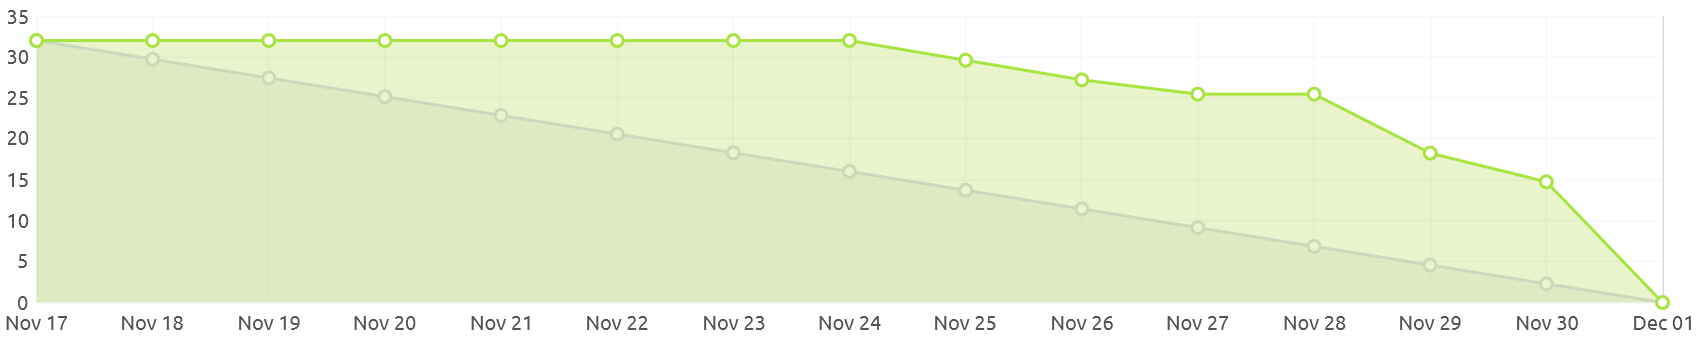
\includegraphics[width=15cm]{./img/sprint3/burndown.png}
    \caption{Burndown}
\end{figure}
\begin{figure}[H]
    \centering
    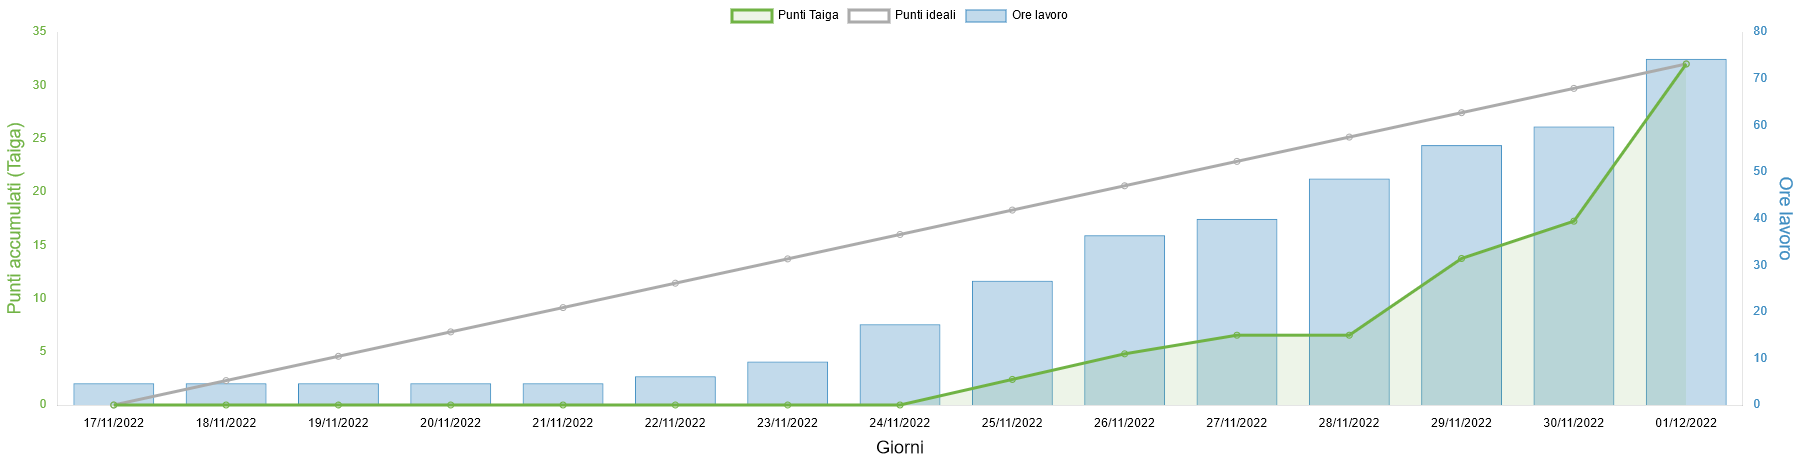
\includegraphics[width=15cm]{./img/sprint3/worktime.png}
    \caption{Progresso dei punti (asse a sinistra) e ore di lavoro (asse a destra)}
\end{figure}

\subsubsection{Retrospettiva}
\begin{figure}[H]
    \centering
    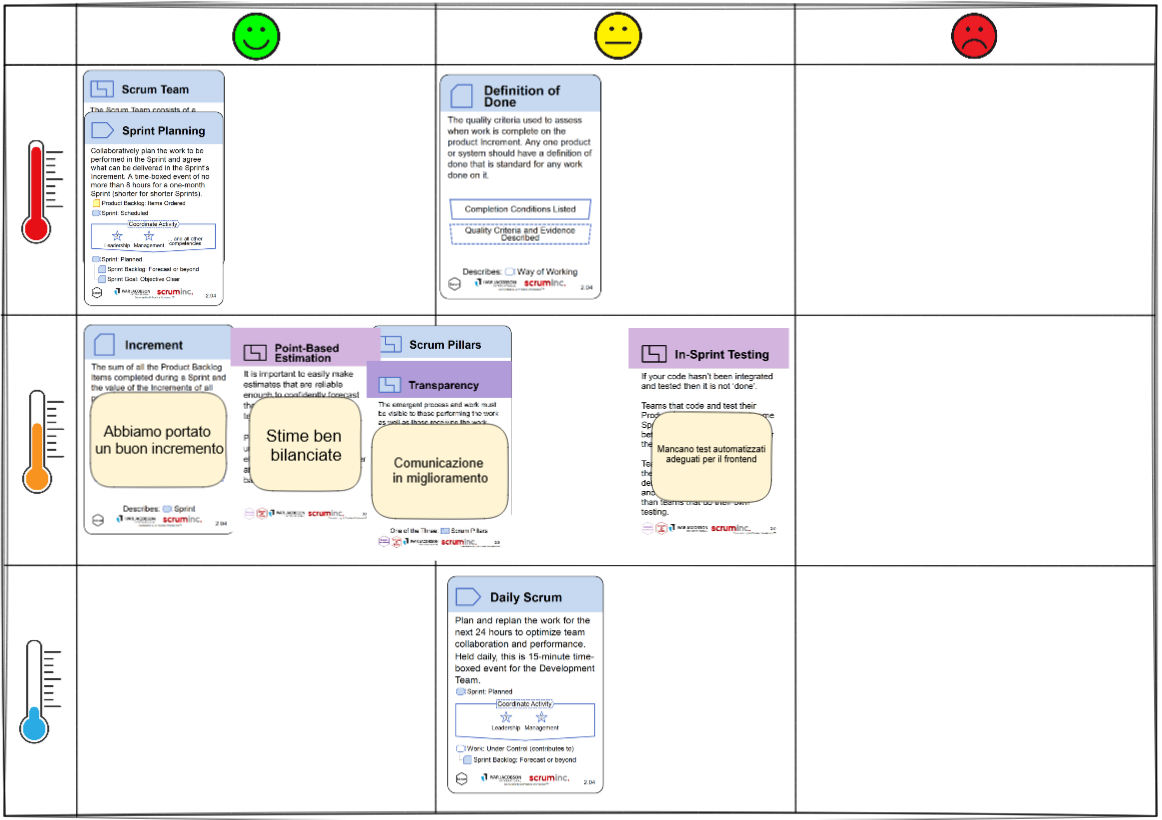
\includegraphics[width=15cm]{./img/sprint3/retrospettiva.png}
    \caption{Pre-retrospettiva del 02/12/2022}
\end{figure}
